% This file was created by tikzplotlib v0.9.8.
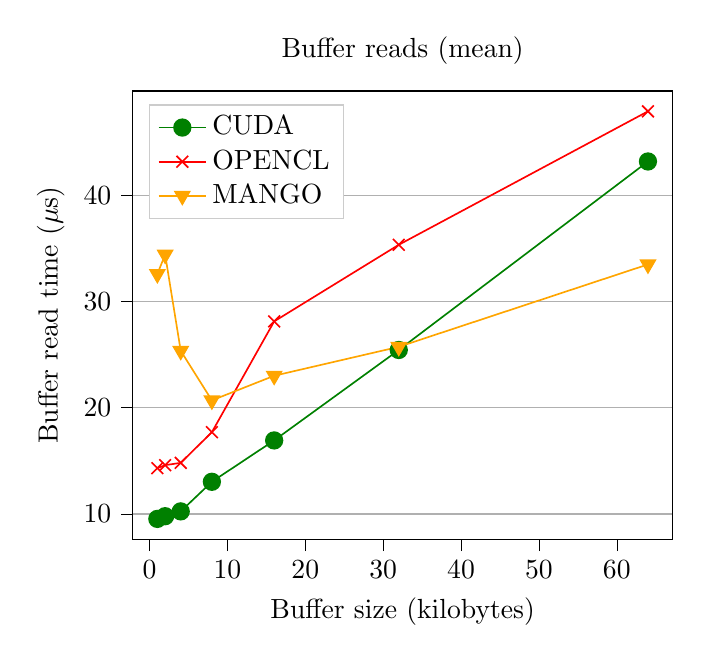
\begin{tikzpicture}

\definecolor{color0}{rgb}{1,0.647058823529412,0}

\begin{axis}[
legend cell align={left},
legend style={
  fill opacity=1,
  draw opacity=1,
  text opacity=1,
  at={(0.03,0.97)},
  anchor=north west,
  draw=white!80!black
},
tick align=outside,
tick pos=left,
title={Buffer reads (mean)},
x grid style={white!69.0196078431373!black},
xlabel={Buffer size (kilobytes)},
xmin=-2.15, xmax=67.15,
xtick style={color=black},
y grid style={white!69.0196078431373!black},
ylabel={Buffer read time ($\mu$s)},
ymajorgrids,
ymin=7.62755214285714, ymax=49.8073641836735,
ytick style={color=black}
]
\addplot [semithick, green!50.1960784313725!black, mark=*, mark size=3, mark options={solid}]
table {%
1 9.54481632653061
2 9.7984693877551
4 10.2500714285714
8 13.03545
16 16.92725
32 25.4355
64 43.1711
};
\addlegendentry{CUDA}
\addplot [semithick, red, mark=x, mark size=3, mark options={solid}]
table {%
1 14.3187777777778
2 14.60112
4 14.8169
8 17.70105
16 28.12495
32 35.3335
64 47.8901
};
\addlegendentry{OPENCL}
\addplot [semithick, color0, mark=triangle*, mark size=3, mark options={solid,rotate=180}]
table {%
1 32.5831616161616
2 34.40658
4 25.3578666666667
8 20.6947894736842
16 23.0111052631579
32 25.7314
64 33.4862
};
\addlegendentry{MANGO}
\end{axis}
\end{tikzpicture}
